\chapter{Gesten}
\label{chap:Gesten}
% Einf\"uhrung
Gestik spiegelt einen wesentlichen Teil unseres Alltags dar. Als Teil der nonverbalen Kommunikation dienen sie zum Ausdruck von Emotionen, zur \"Ubermittlung von Einstellungen, zur Darstellung von Pers\"onlichkeitseigenschaften oder Modulation einer verbalen Nachricht, so Archer und Akert~\cite{bib:archer}. 
\newline
Nachdem bereits die wissenschaftliche Definition einer Gesten nach Kurtenbach und Hulteen in Kapitel~\ref{chap:Einleitung} aufgef\"uhrt wurde und einf\"uhrende Beispiele erl\"autert wurden, werden hier Gesten tiefgehender betrachtet.

\section{Kategorisierung}
Gesten k\"onnen isoliert, oder im Zusammenhang mit einem externen Einfluss oder Objekt existieren. Ein bekanntes Beispiel f\"ur isolierte oder auch freigestellte Gesten, ist die Zeichensprache. In Bezug auf Objekte gibt es eine gro\ss e Bandbreite an m\"oglichen Gesten.
\newline
Daher wurden Gesten in Klassen eingeteilt, um diese besser unterscheiden zu k\"onnen. Die Klassifikation nach Cadoz~\cite{bib:cadoz}, die Gesten nach deren Funktion gruppiert, defniniert drei Typen:
\begin{itemize}
\item \textit{\glslink{Semiotik}{semiotisch}}: Diejenigen Gesten, die aussagekr\"aftige Informationen kommunizieren
\item \textit{\glslink{Ergo}{ergodisch}}: Diejenigen Gesten, die genutzt werden, um das reale Umfeld zu manipulieren und Gegenst\"ande  zu erstellen
\item \textit{\glslink{Epistemik}{epistemisch}}: Diejenigen Gesten, die genutzt werden, um von der Umwelt durch taktile und haptische Erkundung zu lernen
\end{itemize}
Dar\"uber hinaus werden diese Klassen weiter unterteilt. Das Augenmerk dieser Arbeit liegt auf den semiotischen Gesten. Innerhalb dieser Kategorie liefert Mulder~\cite{bib:Mulder} eine weitere Sammlung an verschiedenen Klassifikationen.
\newline
Da der Fokus dieser Arbeit auf der \gls{MCI} liegt, werden vorrangig sogenannte \textit{empty handed} semiotische Gesten betrachtet. Diese k\"onnen entsprechend ihrer Funktionalit\"at weiter unterteilt werden. Rime und Schiaratura~\cite{bib:rime} beschreiben folgende Taxonomie:
\begin{itemize}
\item \textit{symbolische Gesten}: Dabei handelt es sich um Gesten, die innerhalb eines bestimmten Kulturkreises, eine allgemeing\"ultige Bedeutung erlangt haben. Das \enquote{Daumen Hoch}-Zeichen, w\"ahre ein solches Beispiel
\item \textit{\glslink{Deixis}{deiktische} Gesten}: Unter dieser Kategorie fallen Gesten des Zeigens oder der Richtungsweisung. Diese stehen meist in einem Kontext, wie \enquote{Lege das hier hin}
\item \textit{\glslink{Ikoni}{ikonische} Gesten}: Darunter fallen Gesten, die Informationen \"uber Form, Gestalt und Auspr\"agung eines bestimmten Gegenstandes oder einer Handlung
\item \textit{\glslink{Panto}{pantomimische} Gesten}: Dies sind Gesten, die typischer Weise die Nutzung eines nichtgegenw\"artigen Gegenstandes oder Werkzeugs wiederspiegeln. W\"ahrend der Mimik einer Aktion wird dabei eine pantomimische Geste gemacht
\end{itemize}
Baudel und Beaudouin-Lafon~\cite{bib:baudel} zeigen einige Vorteile der Nutzung von symbolischen Gesten zur Interaktion auf:
\begin{itemize}
\item \textit{Nat\"urliche Interaktion}: Gesten sind eine selbstverst\"andliche Form der Interaktion und einfach zu verwenden
\item \textit{Knapp und Ausdrucksstark}: Eine Geste \"ubermittelt genug Information, um Befehl und Paramter zu liefern
\item \textit{Direkte Interaktion}: Einzelne K\"orperteile, insbesondere die Hand, als Eingabeger\"ate machen weitere Signalgeber zwischen Eingabe und Empf\"anger obsolet
\end{itemize}
Nat\"urlich bergen diese auch Nachteile. So k\"onnen symbolische Gesten auf Dauer anstrengend und aufw\"anding werden. Ein Nutzer ben\"otigt in aller Regel Training und ein detailiertes Wissen \"uber Anwendung und Funktion der Gesten, bevor er in der Lage ist, die Anwendung mittels symbolischen Gesten zu bedienen. Je weiter die Anzahl der Gesten und deren Komplexit\"at steigt, desto schwieriger wird es, sich an bestimmte Gesten zu erinnern.
\newline
Weiter stellt sich ein Segmentierungsproblem, dahingehend, dass eine Bewegungsdetektion in aller Regel, den gesamten Verlauf einer Handbewegung, oder die eines anderen K\"orperteils erfasst und die eigentliche Geste nur einen Ausschnitt dieses kontinuierlichen Signalstroms darstellt.
\newline
Es ist daher wichtig, Gesten, die in einer Anwendung verwendet werden sollen, so zu modellieren, dass sie einfach auszuf\"uhren sind, eine angemessene Unterscheidung zwischen diversen Gesten vorhanden ist und diese sich m\"oglichst nahe an nat\"urlichen Bewegungen orientieren.

% jede Geste genau beschreiben - grafik dazu \ldots konzept \ldots realbild von kinect
% hmm modell, genaue beschreibung, stati, \"ubergangsmatrix, zahlen zahlen zahlen
% verkn\"upfung mit aktion f\"ur roboter
\section{Gesten in der Anwendung}

Nachdem bereits in Abschnitt~\ref{subsec:Analyse} die Anforderungen an Gesten ausgef\"uhrt wurden, werden hier die daraus entwickelten Gesten aufgef'\"uhrt. Dabei werden alle grundlegenden Vorgaben f\"ur ein \gls{MCI} aus Abschnitt~\ref{subsec:MCI} ber\"ucksichtigt und die zu entwerfenden Gesten auf Basis der oben beschriebenen Kategorie der \glslink{Semiotik}{semiotischen} Gesten modelliert.

\subsection{Kreisbewegung}
Ein abstrakter Roboter, ist in aller Regel in der Lage, sich im Stand vollst\"andig um seine eigene Achse zu drehen. Dies ist eine hilfreiche Funktion zur Steuerung eines solchen Ger\"ats. Betrachtet man diese Drehung, so findet im Grunde eine Kreisbewegung statt. Um eine intuitive Assoziation zwischen dieser Drehung und der daf\"ur zu verwendeten Geste herzustellen, wird zur Durchf\"uhrung dieser Geste, eine Kreisbewegung verlangt. Das hei\ss t bildlich gesprochen, dass der Bediener mit seinen H\"anden einen Kreis in die Luft zeichnen muss, um die Geste auszuf\"uhren.
\newline
Die Ausf\"uhrung dieser Bewegung ist intuitiv und ohne nennenswerten Trainingsaufwand anwendbar.

\subsubsection{Fachliche Aspekte}
Die Kreisbewegung ist eine \glslink{Ikoni}{ikonische} Geste, da sie die Form eines Kreises wiedergibt. 

\subsubsection{Technische Aspekte}


\begin{figure}[htb]
\centering
\begin{tikzpicture}[
    scale=4,
    axis/.style={very thick, ->, >=stealth'},
    every node/.style={color=black},
    auto,
    ]
    % axis
    \draw[axis] (-1,0)  -- (1.1,0) node(xline)[right]
        {$x$};
    \draw[axis] (-0.5,-0.5) -- (0.5,0.5) node(zline)[above] {$z$};
    % Lines
    \draw[axis] (0,-1) -- (0,1.1) node(yline)[above] {$y$};
    % Lines

\filldraw[fill=gray!5,fill opacity=0.8] (0,0) circle (0.8);

\fill  (0,0.8) circle (.4pt) node[above right]{$S_1$};
\fill  (0.62,0.5) circle (.4pt) node[above right] {$S_2$};
\fill  (0.8,0) circle (.4pt) node[above right] {$S_3$};
\fill  (0.62,-0.5) circle (.4pt) node[ right] {$S_4$};
\fill  (0,-0.8) circle (.4pt) node[above right] {$S_5$};
\fill  (-0.5,-0.62) circle (.4pt) node[above right] {$S_6$};
\fill  (-0.8,0) circle (.4pt) node[above right] {$S_7$};
\fill  (-0.62,0.5) circle (.4pt) node[right] {$S_8$};

\draw [->, thick] (0.05, 0.95) arc (90:-265:0.95);
\end{tikzpicture}
\caption[Abstrakte Darstellung einer Kreisbewegung im Koordinatensystem inklusiver ihrer 8 Zustandspunkte]{Abstrakte Darstellung einer Kreisbewegung im Koordinatensystem inklusiver ihrer 8 Zustandspunkte}
\label{fig:Circle_ideal}
\end{figure}

In einem \acrshort{HMM} wird diese Bewegung durch acht Zust\"ande modelliert. Abbildung~\ref{fig:Circle_ideal} zeigt ein ideales Bild dieser Geste mit ihren acht Zust\"anden.

\begin{figure}[htb]
\centering
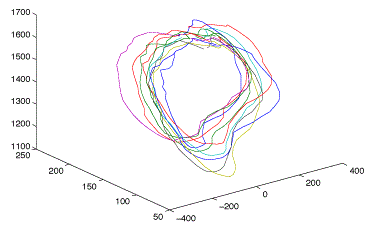
\includegraphics[width=0.5\textwidth]{img/gesture/gesture_circle_real.png}
\caption[Darstellung von Kreisbewegungen im Koordinatensystem die aus realen Trainingsdaten stammen]{Darstellung von Kreisbewegungen im Koordinatensystem die aus realen Trainingsdaten stammen\protect{\footnotemark[1]}}
\label{fig:Circle_reall}
\end{figure}

Diese acht Zust\"ande bilden ein Mittelma\ss dar, um auf der einen Seite kein unterdimensioniertes \gls{HMM} aufzustellen, auf der anderen Seite, aber gen\"ugend Spielraum f\"ur die Akzeptanz von Kreisbewegungen einer etwas ungenauen Form zuzulassen. Abbildung~\ref{fig:Circle_real} zeigt mehrere solcher Kreise, die aus Trainingsdaten ermittelt worden sind.

\footnotetext[1]{Quelle:~\href{http://www.creativedistraction.com/demos/gesture-recognition-kinect-with-hidden-markov-models-hmms/}{\enquote{How to Do Gesture Recognition With Kinect Using Hidden Markov Models (HMMs)}}. creativedistraction.com. Abgerufen Januar 14, 2013}

Die \"Ubergangsmatrix $A$, f\"ur die Geste einer Kreisbewegung wird definiert, als
\begin{equation}
\mathbf{A} = 
\begin{pmatrix}
a_{11} & a_{12} & 0 & 0 & 0 & 0 & 0 & 0 \\
0 & a_{22} & a_{23} & 0 & 0 & 0 & 0 & 0 \\
0 & 0 & a_{33} & a_{34} & 0 & 0 & 0 & 0 \\
0 & 0 & 0 & a_{44} & a_{45} & 0 & 0 & 0 \\
0 & 0 & 0 & 0 & a_{55} & a_{56} & 0 & 0 \\
0 & 0 & 0 & 0 & 0 & a_{66} & a_{67} & 0 \\
0 & 0 & 0 & 0 & 0 & 0 & a_{77} & a_{78} \\
0 & 0 & 0 & 0 & 0 & 0 & 0 & a_{88} \\
\end{pmatrix} \, .
\end{equation}

Dabei ist der \"Ubergangskoeffizient $a_{88}$ gleich $1$. Weiter wird zur Initialisierung f\"ur die weiteren Indizes $i, j$ auf der Hauptiagonalen und der rechten Nebendiagonalen, $a_{ij} = 0,5$ gesetzt. In Trainingsdurchl\"aufen m\"ussen diese Wahrscheinlichkeiten eventuell vereinzelt angepasst werden.

\subsection{Vorw\"artsbewegung}

Die Fortbewegung und die grundlegende Bewegung nach vorne ist die Voraussetzung, damit ein Roboter \"uberhaupt bedient werden kann. Doch diese Bewegung als Befehl zu \"ubergeben, ist wiederum nicht so simpel. Es mehrere M\"oglichkeiten, eine Geste hierf\"ur umzusetzen. Die L\"osung, die hier verwendet wird, basiert auf der Idee der Richtungsanweisung. Das hei\ss t, dem Roboter wird die Anweisung gegeben, sich geradeaus nach vorne zu bewegen.
\newline
Hierbei wird wird ausgehend von der Hand modelliert. Dabei wird ausgehend, von einer K\"orperhaltung, in der die \"uberwachte Hand in N\"ahe des K\"opers auf H\"ohe des Schulterblatts liegt, der Ausgangspunkt festgelegt. Die Aus\"uhrung und Verst\"andlichkeit dieser Geste ist relativ einfach, da sie einfach eine fallende Handbewegung dargestellt. Abbildung~\ref{fig:Forward_ideal} zeigt eine schematische Darstellung mit vier Zust\"anden.

\subsubsection{Fachliche Aspekte}

Die Vorw\"artsbewegung ist eine \glslink{Deixis}{deiktische} Geste, da sie eine Richtungsanweisung wiedergibt. 

\subsubsection{Technische Aspekte}

In einem \acrshort{HMM} wird diese Bewegung durch vier Zust\"ande modelliert. Diese vier Zust\"ande bilden \"ahnlich, wie bei der Kreisbewegung, ein Mittelma\ss dar, ausreichend Spielraum f\"ur die Akzeptanz einer Vorw\"artsbewegung einer etwas ungenauen Form zu besitzen.

\begin{figure}[htb]
\centering
\begin{tikzpicture}[
    scale=4,
    axis/.style={very thick, ->, >=stealth'},
    ]
    % axis
    \draw[axis] (-0.1,0)  -- (1.1,0) node(xline)[right]
        {$x$};
    \draw[axis] (-0.1,-0.1) -- (0.5,0.5) node(zline)[below right] {$z$};
    % Lines
    \draw[axis] (0,-0.1) -- (0,1.1) node(yline)[above] {$y$};
    % Lines

\filldraw[fill=gray!20, fill opacity=0.8] (0,0.8) .. controls (0.1,0.8) and (0.35,0.66) .. (0.48,0.48);
\filldraw[fill=gray!20, draw=gray!20, fill opacity=0.8, draw opacity = 0.8](0,0.8) -- (0.48,0.48) -- ( 0,0);
 \draw  (0.1,0.1) arc (90:10:0.1)  ;
\fill (0.11,0.048) circle (.2pt) ;

 \node[] at (65:0.3)  {$\alpha$};

\fill  (0,0.8) circle (.4pt) node[above right] (a) {$S_1$};
\fill  (0.15,0.74) circle (.4pt) node[above right] {$S_2$};
\fill  (0.35,0.61) circle (.4pt) node[above right] {$S_3$};
\fill  (0.48,0.48) circle (.4pt) node[above right] {$S_4$}
 edge[pil,<-, bend right=60] (a);
\end{tikzpicture}
\caption[Abstrakte Darstellung einer Vorw\"artsbewegung im Koordinatensystem inklusiver ihrer 4 Zustandspunkte]{Abstrakte Darstellung einer  Vorw\"artsbewegung im Koordinatensystem inklusiver ihrer 4 Zustandspunkte}
\label{fig:Foward_ideal}
\end{figure}

Die \"Ubergangsmatrix $A$, f\"ur diese Geste wird definiert, als
\begin{equation}
\mathbf{A} = 
\begin{pmatrix}
a_{11} & a_{12} & 0 & 0\\
0 & a_{22} & a_{23} & 0 \\
0 & 0 & a_{33} & a_{34}\\
0 & 0 & 0 & a_{44} \\
\end{pmatrix} \, .
\end{equation}
Die selben Bedinungen f\"ur die \"Ubergangskoeffizienten gelten f\"ur die Vorw\"artsbewegung, als f\"ur die Kreisbewegung definiert wurden. 
\newline
Der\"Ubergangskoeffizient $a_{44}$ ist gleich $1$. Weiter wird zur Initialisierung f\"ur die weiteren Indizes $i, j$ auf der Hauptiagonalen und der rechten Nebendiagonalen, $a_{ij} = 0,5$ gesetzt. In Trainingsdurchl\"aufen m\"ussen diese Wahrscheinlichkeiten eventuell vereinzelt angepasst werden.

\subsection{Erweiterte Vorw\"artsbewegung}

\begin{figure}[htb]
    \centering
    \subfigure[Darstellung der gesamten erweiterten Vorw\"artsbewegung mit 6 Zust\"anden]
    {
\begin{tikzpicture}[
    scale=4,
    axis/.style={very thick, ->, >=stealth'},
    every node/.style={color=black}
    ]
    % axis
    \draw[axis] (-0.1,0)  -- (1.1,0) node(xline)[right]
        {$x$};
    \draw[axis] (-0.1,-0.1) -- (0.5,0.5) node(zline)[above] {$z$};
    % Lines
    \draw[axis] (0,-0.1) -- (0,1.1) node(yline)[above] {$y$};
    % Lines

\filldraw[fill=gray!5,fill opacity=0.8] (0,0.8) .. controls (0.09,0.78) and (0.3,0.66) .. (0.48,0.48);
\filldraw[fill=gray!5,fill opacity=0.8,draw=gray!20, draw opacity = 0.8] (0,0.8) -- (0.48,0.48) -- (0,0);
 \filldraw[fill=gray!20,fill opacity=0.8]  (0,0) -- (0.5,0.3) arc (0:10:1) ;
    \node[] at (35:0.7)  {$\theta$};

\draw[dashed] (0,0.8) .. controls (0.09,0.78) and (0.3,0.66) .. (0.5,0.3);

 \node[] at (65:0.3)  {$\alpha$};

\fill  (0,0.8) circle (.4pt) node[above right] (a){$S_1$};
\fill  (0.15,0.74) circle (.4pt) node[above right] {$S_2$};
\fill  (0.35,0.61) circle (.4pt) node[above right] {$S_3$};
\fill  (0.48,0.48) circle (.4pt) node[above right] (b){$S_4$}
 edge[pil,<-, bend right=60] (a);
\fill  (0.49,0.4) circle (.4pt) node[below left] {$S_5$};
\fill  (0.5,0.3) circle (.4pt) node[right] {$S_6$}
 edge[pil,<-, bend right=120] (b);
\end{tikzpicture}
\label{fig:forward_first_sub}
    }
    \\
    \subfigure[Detaildarstellung der Seitw\"artsbewegung der erweiterten Vorw\"artsbewegung und ihrer 2 Zust\"ande]
    {
\begin{tikzpicture}[
    scale=4,
    axis/.style={very thick, ->, >=stealth'},
every node/.style={color=black}
    ]
    % axis
    \draw[axis] (-0.1,0)  -- (1.1,0) node(xline)[right]
        {$x$};
    \draw[axis] (-0.1,-0.1) -- (0.5,0.5) node(zline)[above] {$z$};
    % Lines
    \draw[axis] (0,-0.1) -- (0,1.1) node(yline)[above] {$y$};
    % Lines

\draw[dotted] (0,0.8) .. controls (0.09,0.78) and (0.3,0.66) .. (0.48,0.48);
 \filldraw[fill=gray!20,fill opacity=0.8]  (0,0) -- (0.5,0.3) arc (0:10:1) ;
    \node[] at (35:0.7)  {$\theta$};



 \node[] at (60:0.2)  {$\alpha$};

\draw[dashed] (0,0.8) .. controls (0.09,0.78) and (0.3,0.66) .. (0.5,0.3);

\fill  (0.48,0.48) circle (.4pt) node[above right] (a){$S_1$};
\fill  (0.49,0.4) circle (.4pt) node[below left] {$S_2$};
\fill  (0.5,0.3) circle (.4pt) node[right] {$S_3$}
 edge[pil,<-, bend right=80] (a);
\end{tikzpicture}
\label{fig:forward_second_sub}
}
\caption{Idealisierte Darstellung der 1. Variante einer erweiterten Vorw\"artsbewegung mit 6 Zust\"anden}
    \label{fig:Forward_ideal_var1}
\end{figure}

Die oben beschriebene Vorw\"artsbewegung beinhaltet keine Information \"uber einen Winkel, in dem sich der Roboter fortbewegen soll. Um diese Information zu erhalten, muss die Geste und das darunterliegende \acrshort{HMM} angepasst und erweitert werden.
\newline
\begin{equation}
\mathbf{A} = 
\begin{pmatrix}
a_{11} & a_{12} & 0 & 0\\
0 & a_{22} & a_{23} & 0\\
0 & 0 & a_{33} & a_{34}\\
0 & 0 & 0 & a_{44} \\
\end{pmatrix} \, .
\end{equation}
Die selben Bedinungen f\"ur die \"Ubergangskoeffizienten gelten f\"ur die Vorw\"artsbewegung, als f\"ur die Kreisbewegung definiert wurden. 
\newline
Der\"Ubergangskoeffizient $a_{44}$ ist gleich $1$. Weiter wird zur Initialisierung f\"ur die weiteren Indizes $i, j$ auf der Hauptiagonalen und der rechten Nebendiagonalen, $a_{ij} = 0,5$ gesetzt. In Trainingsdurchl\"aufen m\"ussen diese Wahrscheinlichkeiten eventuell vereinzelt angepasst werden.\begin{equation}
\mathbf{A} = 
\begin{pmatrix}
a_{11} & a_{12} & 0 & 0\\
0 & a_{22} & a_{23} & 0\\
0 & 0 & a_{33} & a_{34}\\
0 & 0 & 0 & a_{44} \\
\end{pmatrix} \, .
\end{equation}
Die selben Bedinungen f\"ur die \"Ubergangskoeffizienten gelten f\"ur die Vorw\"artsbewegung, als f\"ur die Kreisbewegung definiert wurden. 
\newline
Der\"Ubergangskoeffizient $a_{44}$ ist gleich $1$. Weiter wird zur Initialisierung f\"ur die weiteren Indizes $i, j$ auf der Hauptiagonalen und der rechten Nebendiagonalen, $a_{ij} = 0,5$ gesetzt. In Trainingsdurchl\"aufen m\"ussen diese Wahrscheinlichkeiten eventuell vereinzelt angepasst werden.

\begin{figure}[htb]
\centering
\begin{tikzpicture}[
    scale=4,
    axis/.style={very thick, ->, >=stealth'},
every node/.style={color=black}
    ]
    % axis
    \draw[axis] (-0.1,0)  -- (1.1,0) node(xline)[right]
        {$x$};
    \draw[axis] (-0.1,-0.1) -- (0.5,0.5) node(zline)[above] {$z$};
    % Lines
    \draw[axis] (0,-0.1) -- (0,1.1) node(yline)[above] {$y$};
    % Lines

\filldraw[fill=gray!20, fill opacity=0.8] (0,0.8) .. controls (0.09,0.78) and (0.3,0.66) .. (0.5,0.3);
\filldraw[fill=gray!20,fill opacity=0.8,draw=gray!20, draw opacity = 0.8](0,0.8) -- (0.5,0.3) -- ( 0,0);
\draw[dotted] (0,0.8) .. controls (0.09,0.78) and (0.3,0.66) .. (0.48,0.48);
 \draw  (0,0) -- (0.5,0.3) arc (0:10:1) ;
    \node[] at (35:0.7)  {$\theta$};


 \node[] at (60:0.2)  {$\alpha$};

\fill  (0,0.8) circle (.4pt) node[above right] (a){$S_1$};
\fill  (0.17,0.7) circle (.4pt) node[above right] {$S_2$};
\fill  (0.35,0.53) circle (.4pt) node[above right] {$S_3$};
\fill  (0.5,0.3) circle (.4pt) node[below right] {$S_4$}
 edge[pil,<-, bend right=80] (a);
\end{tikzpicture}
\caption[Idealisierte Darstellung der 2. Variante einer erweiterten Vorw\"artsbewegung mit 4 Zust\"anden]{Idealisierte Darstellung der 2. Variante einer erweiterten Vorw\"artsbewegung mit 4 Zust\"anden}
\label{fig:Forward_ideal_var2}
\end{figure}

Dabei gibt es zwei Varianten, wie diese Information exktrahiert werden kann. Variante 1, siehe Abbildung~\ref{fig:Forward_ideal_var1}, zeigt, wie an die bestehende Geste eine weitere Bewegung angef\"ugt wird, um die Winkelinformation $\theta$ zuerhalten, Variante 2, siehe Abbildung~\ref{fig:Forward_ideal_var2} , eine \"uberarbeitete Geste, in der der Winkel $\theta$ direkt \"uber das Koordinatensystem extrapoliert wird.
\newline
Variante 2 stellt sich unter realen Testbedinungen als Problemanf\"allig und ungenau heraus, da bereits bei der Gestenerkennung eine gewisse Unsch\"arfe vorherrscht. Der Winkel $\theta$ wird dabei also verf\"alscht wiedergegeben und es kann nicht sichergestellt werden, dass die Intention des Bedieners vollst\"andig in die Informationen, die die Geste an den Roboter liefert einflie\ss t. Daher wird diese Variante nicht weiter verfolgt.
\newline
Variante 1 kann anschaulich in zwei Teile zerlegt werden. Neben Abbildung~\ref{fig:forward_first_sub}, die den gesamten Ablauf zeigt, weisst Abbildung~\ref{fig:forward_second_sub} auf den zweiten Teil hin, der die Geste dahingehend erweitert, dass mit einer relativen Genauigkeit, der Winkel $\theta$ aus der Geste ausgelesen werden kann. Die Gr\"o\ss e des Winkels, oder die Geschwindigkeit, mit der die Geste ausgef\"uhrt wird, spielt keine besondere Rolle, denn sobald das \acrshort{HMM} entsprechend trainiert wurde, wird die Geste in aller Regel, verl\"asslich erkannt.

\subsubsection{Technische Aspekte der Variante 1}
Ausgehend von der vorhandenen Vorw\"artsbewegung und kann das \acrshort{HMM} der erweiterten 
Vorw\"artsbewegung und deren \"Ubergangsmatrix $A$ definiert werden, als
\begin{equation}
\mathbf{A} = 
\begin{pmatrix}
a_{11} & a_{12} & 0 & 0 & 0 & 0 & \\
0 & a_{22} & a_{23} & 0 & 0 & 0 & \\
0 & 0 & a_{33} & a_{34} & 0 & 0 & \\
0 & 0 & 0 & a_{44} & a_{45} & 0 & \\
0 & 0 & 0 & 0 & a_{55} & a_{56} & \\
0 & 0 & 0 & 0 & 0 & a_{66} \\
\end{pmatrix} \, .
\end{equation}

Dabei ist der \"Ubergangskoeffizient $a_{66}$ gleich $1$. Weiter wird zur Initialisierung f\"ur die weiteren Indizes $i, j$ auf der Hauptiagonalen und der rechten Nebendiagonalen, $a_{ij} = 0,5$ gesetzt. In Trainingsdurchl\"aufen m\"ussen diese Wahrscheinlichkeiten eventuell vereinzelt angepasst werden.

\subsection{Haltesignal}

\begin{figure}[htb]
    \centering
    \subfigure[Abstrakte Darstellung des Haltesignals aus einer m\"oglichen Vorwz"artsbewegung heraus, mit ihren 4 Zust\"anden]
    {
	
\begin{tikzpicture}[
    scale=4,
    axis/.style={very thick, ->, >=stealth'},
every node/.style={color=black}
    ]
    % axis
    \draw[axis] (-0.1,0)  -- (1.1,0) node(xline)[right]
        {$x$};
    \draw[axis] (-0.1,-0.1) -- (0.5,0.5) node(zline)[above] {$z$};
    % Lines
    \draw[axis] (0,-0.1) -- (0,1.1) node(yline)[above] {$y$};
    % Lines

\filldraw[fill=gray!20, fill opacity=0.8] (0,0.8) .. controls (0.09,0.78) and (0.3,0.66) .. (0.5,0.3);
\filldraw[fill=gray!20,fill opacity=0.8,draw=gray!20, draw opacity = 0.8](0,0.8) -- (0.5,0.3) -- ( 0,0);
\draw[dotted] (0,0.8) .. controls (0.09,0.78) and (0.3,0.66) .. (0.48,0.48);
 \draw  (0,0) -- (0.5,0.3) arc (0:10:1) ;
    \node[] at (35:0.7)  {$\theta$};


 \node[] at (60:0.2)  {$\alpha$};


\fill  (0,0.8) circle (.4pt) node[above right] (a){$S_1$};
\fill  (0.17,0.7) circle (.4pt) node[above right] {$S_2$};
\fill  (0.35,0.53) circle (.4pt) node[above right] {$S_3$};
\fill  (0.5,0.3) circle (.4pt) node[below right] {$S_4$}
 edge[pil,->, bend right=80] (a);
\end{tikzpicture}
        \label{fig:halt_first_sub}
    }
    \\
    \subfigure[Abstrakte Darstellung des Haltesignals aus einer m\"oglichen Kreisbewegung heraus, mit ihren 4 Zust\"anden]
    {
\begin{tikzpicture}[
    scale=4,
    axis/.style={very thick, ->, >=stealth'},
every node/.style={color=black}
    ]
    % axis
    \draw[axis] (-0.1,0)  -- (1.1,0) node(xline)[right]
        {$x$};
    \draw[axis] (-0.1,-0.1) -- (0.5,0.5) node(zline)[above] {$z$};
    % Lines
    \draw[axis] (0,-0.1) -- (0,1.1) node(yline)[above] {$y$};
    % Lines

\draw (0.5,1.1) -- (0,0.8);
\draw[dotted] (0.5,1.1) -- (1,1.1) -- (0,0.8);
 \draw[dashed]  (0,0.8) -- (0.34,1) arc (60:53.5:1) -- (0,0.8) ;
    \node[] at (65:1.1)  {$\theta$};
\filldraw[fill=gray!20,fill opacity=0.8,draw=gray!20, draw opacity = 0.8](0,0.8) -- (0.5,1.1) --  (1,1.1);

\fill  (0.5,1.1) circle (.4pt) node[above right] (a){$S_1$};
\fill (0.34,1) circle (.4pt) node[above] {$S_2$};
\fill  (0.2,0.92) circle (.4pt) node[above] {$S_3$};
\fill (0,0.8)  circle (.4pt) node[above right] {$S_4$}
 edge[pil,<-, bend left=80] (a);
\end{tikzpicture}
        \label{fig:halt_second_sub}
    }
  
    \caption{Abstrakte Darstellung der Modelle f\"ur die Geste des Haltesignals mit jeweils 4 Zust\"anden}
    \label{fig:halt_ideal}
\end{figure}

Die M\"oglichkeit den Roboter anzuhalten ist die wichtigste Funktion, da hierbei die Sicherheit vor Unf\"allen eine wesentliche Rolle spielt. Der Roboter muss m\"oglichst schnell und einfach zu stoppen sein. Sei es einfach aus dem Grund, dass der Bediener seine Aufgabe abgeschlossen hat, oder der nicht unerhebliche Fall der Unfallvermeidung oder Sicherstellung des Robots eintritt.
\newline
Auf Basis dieses Sicherheitsgedanken wurde das Haltesignal modelliert und hierzu die menschliche Haltung bei Gefahr betrachtet. Der Mensch tritt bei drohender Gefahr in eine defensive Stellung, tritt einen Schritt zur\"uck, oder zieht Gelenke, wie Arme oder Beine n\"aher zum K\"orperschwerpunkt.
\newline
Um die Erkennung der Geste zu optimieren und auch in den verschiedenen Startzust\"anden zu erkennen zeigt die Abbildung~\ref{fig:halt_ideal}, zwei abstrakte Modelle mit ensprechenden Zust\"anden. 
\newline
Abbildung~\ref{fig:halt_first_sub} zeigt, wie ein Haltesignal aus einer Vorw\"artsbewegung heraus erzeugt werden. Dabei spielt der Winkel $\theta$ nur dann eine Rolle, wenn er sich w\"ahrend der laufenden Geste stark \"andert, da dann nicht mehr sichergestellt ist, ob diese Geste \"uberhaubt beabsichtigt war.
\newline
In Abbildung~\ref{fig:halt_second_sub} is dargestellt, wie aus einer Kreisbewegung in das Haltesignal \"ubergegangen wird. Dabei ist der Winkel $\theta$ ebenfalls nur dann relevant, sofern zweifeln an der Intention der Geste besteht, da dieser sich \"andert.

\subsubsection{Fachliche Aspekte}
Das Haltesignal ist eine \glslink{Panto}{pantomimische} Geste, da sie den Schutgedanken wiedergibt und hierbei die Emotion in eine defenisve Bewegung oder Haltung resultiert. 

\subsubsection{Technische Aspekte}
Die Geste f\"ur das Haltesignal daran angelehnt, so ausgef\"uhrt, dass der Bediener mindestens eine Hand zum K\"orper zur\"uckziehen muss. Eine abstrakte Ansicht hierzu liefert die Abbildung~\ref{fig:Hold_ideal}. Mittels vier Zust\"anden wird hier ein \acrshort{HMM} modelliert.
\newline
Wichtig hierbei ist, dass der Bediener sich zum Start des Haltesignals gerade in einer Vorw\"artsbewegung, oder einer Kreisbewegung befinden kann. Daher werden, wie in Abbildung~\ref{fig:Hold_ideal} zu sehen, zwei Varianten erkannt und akzeptiert. F\"ur die \"Ubergangsmatrix $A$ hat das keine Auswirkung, diese ist f\"ur beide F\"alle definiert, als
\begin{equation}
\mathbf{A} = 
\begin{pmatrix}
a_{11} & a_{12} & 0 & 0\\
0 & a_{22} & a_{23} & 0\\
0 & 0 & a_{33} & a_{34}\\
0 & 0 & 0 & a_{44} \\
\end{pmatrix} \, .
\end{equation}
Die selben Bedinungen f\"ur die \"Ubergangskoeffizienten, wie zuvor, gelten auch hier, jedoch mit einer wichtigen Ausnahme: Der\"Ubergangskoeffizient $a_{44}$ ist gleich $1$. Weiter wird zur Initialisierung f\"ur die weiteren Indizes $i, j$ auf der Hauptiagonalen und der rechten Nebendiagonalen, $a_{ij} = 0,5$ gesetzt. In Trainingsdurchl\"aufen m\"ussen diese Wahrscheinlichkeiten eventuell vereinzelt angepasst werden. Die Beobachtungsfolge $O = O_1\, O_2\, O_3\, O_4$ besteht bei den zwei Varianten, jedoch aus verschiedenen Zust\"anden $S_1, S_2, S_3, S_4$.

\subsection{Entriegeln --- Blockieren}

Eine zur Steuerung eines Roboters nicht notwendige, dennoch recht n\"utzliche Geste zur Entriegelung und Blockierung weiterer Gesteneingaben. Dem Bediener, auf der einen Seite, wird ein gewisser Komfort dadurch geboten, dass er nicht st\"andig gegenw\"artig und bewusst darauf achten muss, nat\"urliche Bewegungen nicht mit Gestenbefehlen zu vermischen. Auf der anderen Seite erlangt das gesamte System der Anwendung dabei an Stabilit\"at, da Fehleingaben des Nutzers minimiert werden.
\newline
Angelehnt an ein Schiebeschloss muss hierbei ledigliche entweder eine Handbewegung von links nach rechts (zum Blockieren), wie in Abbildung~\ref{fig:Lock_ideal} dargestellt, als auch eine Handbewegung von rechts nach links (zum Entriegeln) ausgef\"uhrt werden.

\begin{figure}[htb]
\centering
\begin{tikzpicture}[
    scale=4,
    axis/.style={very thick, ->, >=stealth'},
    every node/.style={color=black},
node distance=1cm, auto,
    ]
    % axis
    \draw[axis] (-0.1,0)  -- (1.1,0) node(xline)[right]
        {$x$};
    \draw[axis] (-0.1,-0.1) -- (0.5,0.5) node(zline)[above] {$z$};
    % Lines
    \draw[axis] (0,-0.1) -- (0,1.1) node(yline)[above] {$y$};
    % Lines

\draw (0,0.8) --  (1,0.8);

\fill  (0,0.8) circle (.4pt) node[above right] (a){$S_1$} ;
\fill  (0.25,0.8) circle (.4pt) node[above right] {$S_2$} ;
\fill  (0.5,0.8) circle (.4pt) node[above right] {$S_3$} ;
\fill  (0.75,0.8) circle (.4pt) node[above right] {$S_4$} ;
\fill  (1,0.8) circle (.4pt) node[above right] {$S_5$}
 edge[pil,<->,  bend right] (a) ;
\end{tikzpicture}
\caption[Idealisierte Darstellung der Geste zum Blockieren und Freigeben der Gesteneingabe mit 4 Zust\"anden]{Idealisierte Darstellung der Geste zum Blockieren und Freigeben der Gesteneingabe mit 4 Zust\"anden}
\label{fig:Lock_ideal}
\end{figure}

\subsubsection{Fachliche Aspekte}
Das Entriegeln --- Blockieren ist eine \glslink{Panto}{pantomimische} Geste, da sie das Werkzeug \textit{Schloss} nachmiemt. 

\subsubsection{Technische Aspekte}
Das besondere an dieser Geste, ist die Tatsache, dass sie von beiden Richtungen aus durchgef\"uhrt werden kann und dabei unterschiedliche Aktionen ausf\"uhrt.
\newline
Daher verh\"alt sich die \"Ubergangsmatrix $A$ anders, als dies bisher der Fall ist. Zus\"atzlich zur rechten Nebendiagonalen ist hier auch die linke Nebendiagonale mit Koeffizienten $a_{ij}$ besetzt. Demnach ist die Matrix definiert, als
\begin{equation}
\mathbf{A} = 
\begin{pmatrix}
a_{11} & a_{12} & 0 & 0\\
 a_{21} & a_{22} & a_{23} & 0\\
0 &  a_{32} & a_{33} & a_{34}\\
0 & 0 & a_{43} & a_{44} \\
\end{pmatrix} \, .
\end{equation}
Der\"Ubergangskoeffizient $a_{44}$ ist hier ungleich $1$, da er nicht nur Endpunkt, sondern auch Start der Geste sein kann. Daher werden zur Initialisierung f\"ur alle Indizes $i, j$ auf der Hauptiagonalen und den Nebendiagonalen, $a_{ij} = 0,5$ gesetzt. In Trainingsdurchl\"aufen m\"ussen diese Wahrscheinlichkeiten eventuell vereinzelt angepasst werden, um insbesondere $a_{11}$ und $a_{44}$ optimal zu bestimmen. Die Beobachtungsfolge $O = O_1\, O_2\, O_3\, O_4$ besteht bei den zwei Varianten ($\Leftarrow, \Rightarrow$), jedoch aus den umgedrehten Zustandensfolgen $S_1\, S_2\, S_3\, S_4 (\Rightarrow)$ und $S_4\, S_3\, S_2\, S_1 (\Leftarrow)$.